
\begin{itemize}
	\item \textbf{Investigue sobre topologías de antenas adecuadas para lograr su objetivo considerando el tamaño total de la estructura y el espacio disponible en el reflector.}\\\\
	Se busca investigar diferentes topologias con el fin de lograr una antena direccional, compacta y que opere en el rango de frecuencias de 3.3 y 3.5[Ghz], algunas de estas son:
	\begin{itemize}
		\item \textbf{Antena Horn (Bocina):} Antena eficiente y común para alimentar un reflector parabólico, ofreciendo un patrón de radiación uniforme y polarización lineal. Su diseño consiste en una apertura que minimiza reflexiones internas, aunque su tamaño puede ser voluminoso. Ideal para frecuencias de 3.3 a 3.5 GHz, con dimensiones de aproximadamente 9 cm.
		
		\item \textbf{Antena Patch:} Antena compacta y ligera utiliza un parche metálico sobre un sustrato dieléctrico, siendo fácil de fabricar e integrar en sistemas modernos. Aunque menos direccional que la horn, su polarización lineal y tamaño reducido la hacen adecuada para reflectores pequeños o medianos.
		
		\item \textbf{Antena Helicoidal:} Configurada en modo axial, puede proporcionar polarización lineal y un haz direccional bien definido. Es eficiente para aplicaciones de microondas en 3.3 a 3.5 GHz, aunque su construcción es más compleja y su tamaño mayor que otras opciones compactas.
		
		\item \textbf{Cantenna:} Basada en una guía de onda cilíndrica, esta antena es económica y fácil de construir, utilizando una lata común como base. Optimizada para la banda de operación, ofrece un buen desempeño en ganancia y polarización lineal.
	\end{itemize}
	
	Analizando todos estos tipos de antena que pueden ser util para el proposito buscado se decidio optar por la antena Horn de bocina
	\item \textbf{Diseñe su alimentador en HFSS parametrizando sus dimensiones relevantes.}\\
	En base a los tipos de antenas visto anteriormente se opto por la antena Horn de bocina, la cual se diseño en HFSS, pero primero se debe caracterizar las dimensiones, por lo que se tiene el siguiente esquema
	\begin{figure}[H]
		\centering
		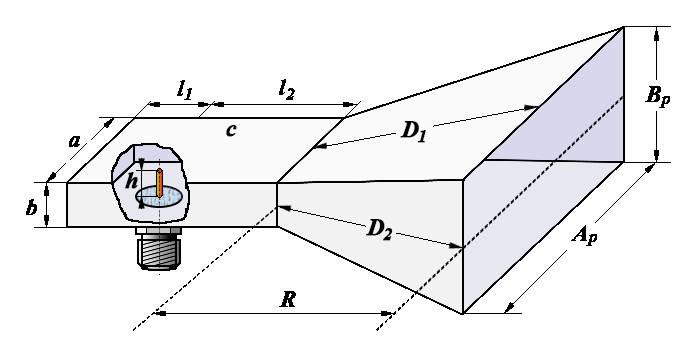
\includegraphics[width=0.55\textwidth]{img/ejemplos/Figure_1}
		\caption{Esquema de la antena con las medidas de sus parametros mas relevantes}
	\end{figure}
	De manera teorica se procede a obtener los valores de las dimensiones de la guia de onda y el cuerno, los cuales se muestran en la tabla \ref{tab:waveguide_horn}
	\begin{table}[H]
		\centering
		\begin{tabular}{|l|l|}
		\hline
		\textbf{Parámetro}                                   & \textbf{Medida}              \\ \hline
		Dimensiones de la apertura del cuerno (Ap×Bp)       & 152 mm × 95.5 mm            \\ \hline
		Longitud del cuerno (R)                             & 46.3 mm                     \\ \hline
		Longitud del plano ancho del cuerno (D1)            & 56.2 mm                     \\ \hline
		Longitud del plano angosto del cuerno (D2)          & 62.7 mm                     \\ \hline
		Altura del pin excitador (h)                        & 21.5 mm                     \\ \hline
		Distancia del pin a la pared trasera de la guía (l1)& 16.9 mm                     \\ \hline
		Distancia del pin a la garganta del cuerno (l2)     & 55.3 mm                     \\ \hline
		Rango de frecuencias (f)                            & 3.3 GHz - 3.5 GHz         \\ \hline
		Ancho de banda ($\Delta f$)                         & 200 MHz                     \\ \hline
		\end{tabular}
		\caption{Resumen de medidas de la guía de onda y el horn.}
		\label{tab:waveguide_horn}
		\end{table}
	Posteriormente se modela en HFSS obteniendo el siguiente modelo 3D de la antena:
	\begin{figure}[H]
		\centering
		% Primera subfigura
		\begin{subfigure}[b]{0.45\textwidth}
			\centering
			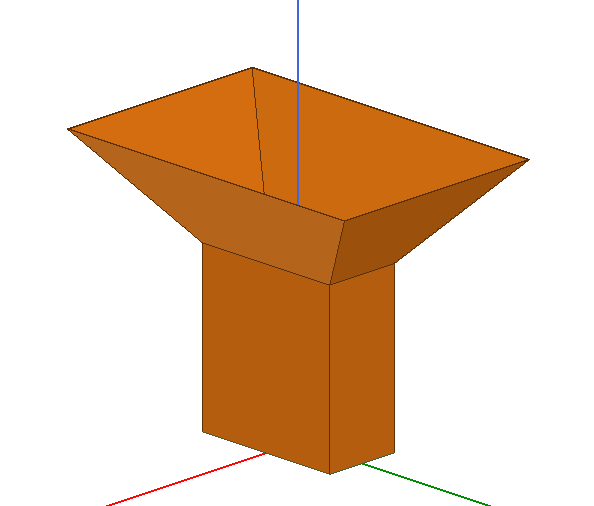
\includegraphics[width=0.8\textwidth]{img/ejemplos/Figure_2}
			\caption{Vista isometrica del modelo 3D de la antena en HFSS}
			\label{fig:Imagen-Madrid}
		\end{subfigure}
		\hfill
		% Segunda subfigura
		\begin{subfigure}[b]{0.45\textwidth}
			\centering
			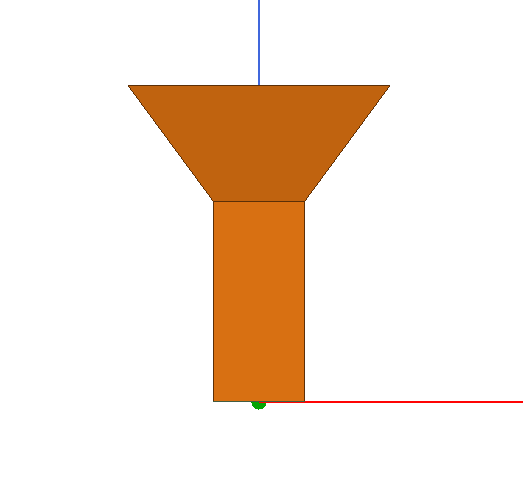
\includegraphics[width=0.85\textwidth]{img/ejemplos/Figure_3}
			\caption{Vista lateral del modelo 3D de la antena en HFSS}
			\label{fig:Imagen-Londres}
		\end{subfigure}
		\caption{Antena Horn modelada en HFSS}
		\label{fig:Figura-Ciudades}
	\end{figure}
	La antena no presenta resultados satisfactorios tanto en sus parametros $S_{11}$ como en el patron de radiacion, por lo que se deben optimizar sus valores
	\newpage
	\item \textbf{Realice un Parametric sweep o use el optimizador para mejorar el desempeño de su
	antena.}\\\\
	Dado que se busca mejorar el desempeño de la antena, se procede a realizar un analisis de optimizacion en HFSS, para ello se varian los valores vistos en la tabla \ref{tab:waveguide_horn} y se obtiene el siguientes resultados:
	\begin{table}[H]
		\centering
		\begin{tabular}{|l|l|}
		\hline
		\textbf{Parámetro}                                   & \textbf{Medida}              \\ \hline
		Dimensiones de la apertura del cuerno (Ap×Bp)       & 149 mm × 97.8 mm            \\ \hline
		Longitud del cuerno (R)                             & 44.5 mm                     \\ \hline
		Longitud del plano ancho del cuerno (D1)            & 53.9 mm                     \\ \hline
		Longitud del plano angosto del cuerno (D2)          & 60.2 mm                     \\ \hline
		Altura del pin excitador (h)                        & 20.1 mm                     \\ \hline
		Distancia del pin a la pared trasera de la guía (l1)& 17.8 mm                     \\ \hline
		Distancia del pin a la garganta del cuerno (l2)     & 57.5 mm                     \\ \hline
		Rango de frecuencias (f)                            & 3.3 GHz - 3.5 GHz         \\ \hline
		Ancho de banda ($\Delta f$)                         & 200 MHz                     \\ \hline
		\end{tabular}
		\caption{Resumen de medidas optimizadas}
		\label{tab:waveguide_horn_adjusted}
		\end{table}
		Posterioremente se grafica el parametro $S_{11}$ ademas de su patron de radiacion:
		\begin{figure}
			\centering
			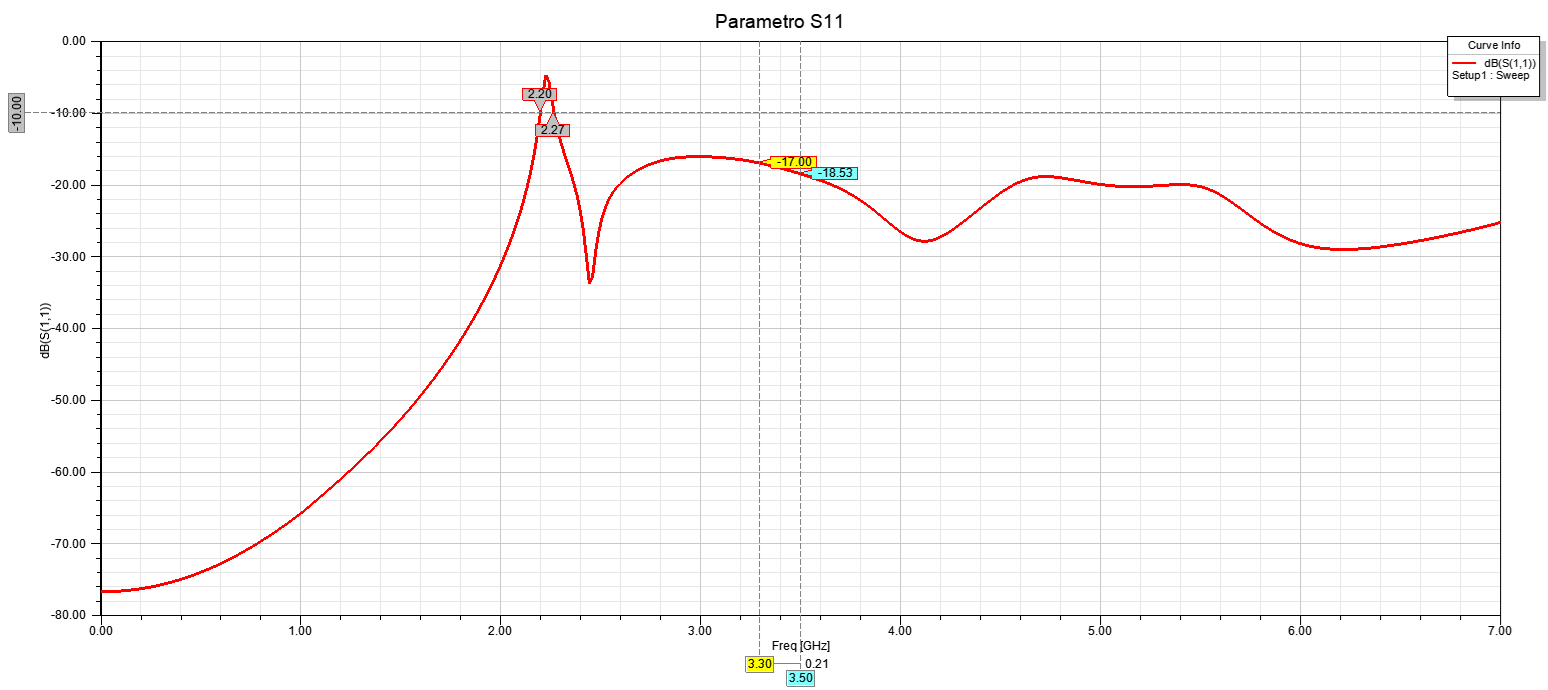
\includegraphics[width=1\textwidth]{img/ejemplos/Figure_4}
			\caption{Parametro $S_{11}$ de la antena optimizada}
		\end{figure}
		\begin{figure}
			\centering
			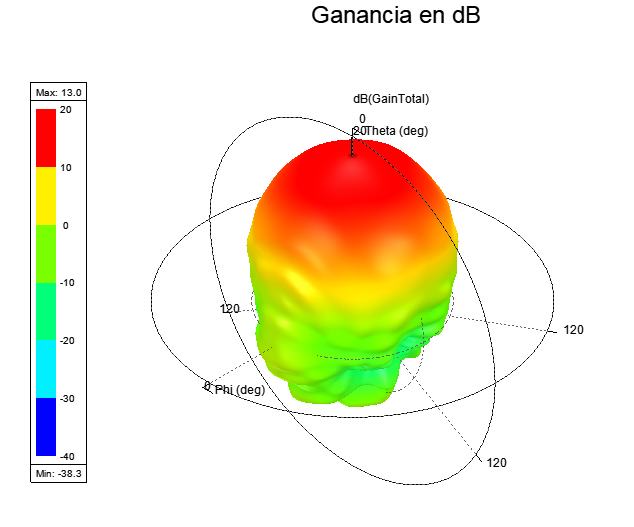
\includegraphics[width=0.6\textwidth]{img/ejemplos/Figure_5}
			\caption{Ganancia de la antena optimizada en dB} 
		\end{figure}
		\begin{figure}
			\centering
			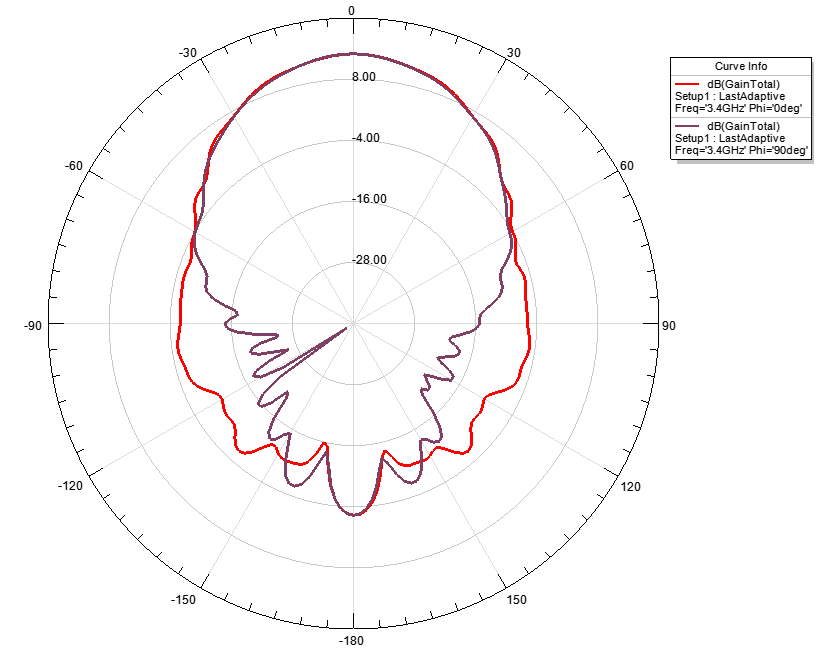
\includegraphics[width=0.6\textwidth]{img/ejemplos/Figure_6}
			\caption{Patron de radiacion de la antena optimizada}
		\end{figure}
		Finalmente se concluye que el rendimiento simulado es suficiente para cumplir con los requerimientos del proyecto por lo que se procede a la fabricacion de la antena.
		\newpage
		\item \textbf{Construya la antena utilizando materiales de su preferencia.}\\\\
		Para la fabricacion de la antena se recurrio a materiales de facil acceso y bajo costo, por lo que se opto por el uso de impresion 3D para la fabricacion de la antena, y posteriormente se recubrio con una capa de cobre por el interior, ademas del espacio para la alimentacion, esto se visualiza:
		\begin{figure}[H]
			\centering
			% Primera subfigura
			\begin{subfigure}[b]{0.45\textwidth}
				\centering
				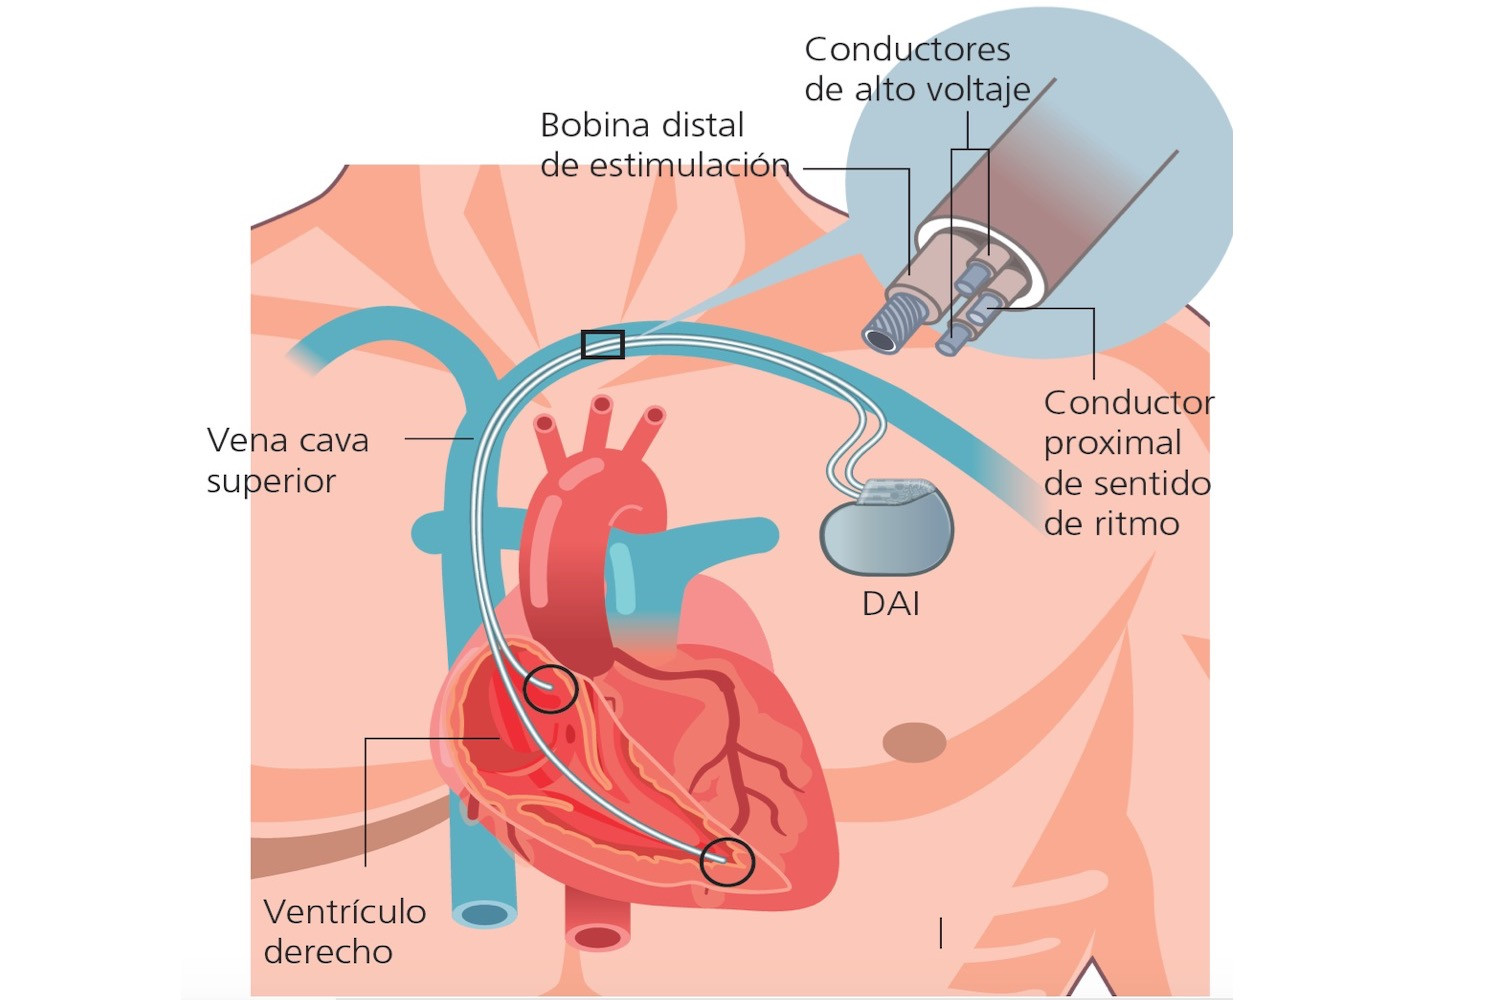
\includegraphics[width=1\textwidth]{img/ejemplos/Figure_7}
				\caption{Vista frontal de la antena fabricada, donde se observa el pin central de alimentacion , ademas del recubrimiento de cobre}
				\label{fig:antena_cobre1}
			\end{subfigure}
			\hfill
			% Segunda subfigura
			\begin{subfigure}[b]{0.45\textwidth}
				\centering
				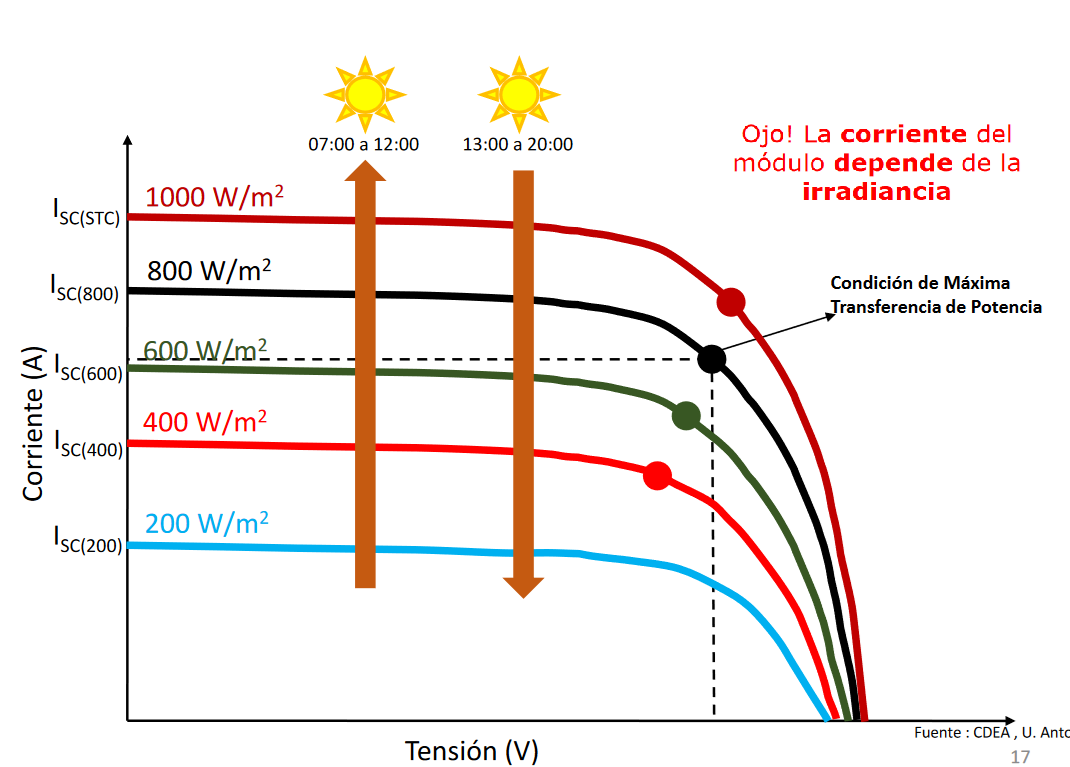
\includegraphics[width=1\textwidth]{img/ejemplos/Figure_8}
				\caption{Vista isometrica de la antena fabricada, donde se observa la conexion y el modelado}
				\label{fig:antena_cobre2}
			\end{subfigure}
			\caption{Visualizacion de la antena fabricada con impresion 3D y recubrimiento de cobre}
			\label{fig:antenacobre1}
		\end{figure}
		Se obtienen resultados satisfactorios, debido a su rigidez y se testea la conductividad en todas las caras funcionando de manera correcta.
		\newpage
		\item \textbf{Mida las reflexiones (solo alimentador) en el puerto de entrada. Estas deben ser menores que -10dB en la frecuencia de operación. Grafique las reflexiones medidas y simuladas. De ser necesario, modifique las dimensiones para mejorar el rendimiento}\\\\
		Se procede a medir las reflexiones en el puerto de entrada de la antena, obteniendo los siguientes resultados:
		\begin{figure}
			\centering
			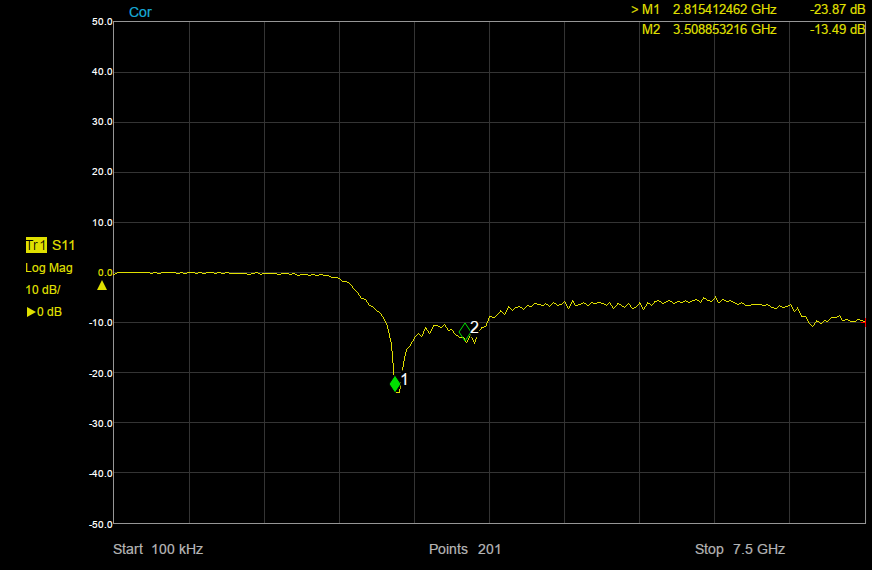
\includegraphics[width=0.6\textwidth]{img/ejemplos/Figure_9}
			\caption{Reflexiones medidas ($S_{11}$)en el puerto de entrada de la antena}
		\end{figure}
		Se observan que las reflexiones cumplen con los requerimientos de -10dB en la frecuencia de operacion. Es importante el destacar que se modifico la altura del pin central acortandolo un par de milimetros, lo que se reflejo un mejor rendimiento en la antena.
		\newpage
		\item \textbf{Mida el patrón de radiación de su alimentador (ambos planos E y H) considerando un radioenlace copolarizado. Grafique sus resultados}\\\\
		Se busca el graficar el patron de radiacion de la antena, para ambos planos E y H, obteniendo los siguientes resultados:
		\begin{figure}
			\centering
			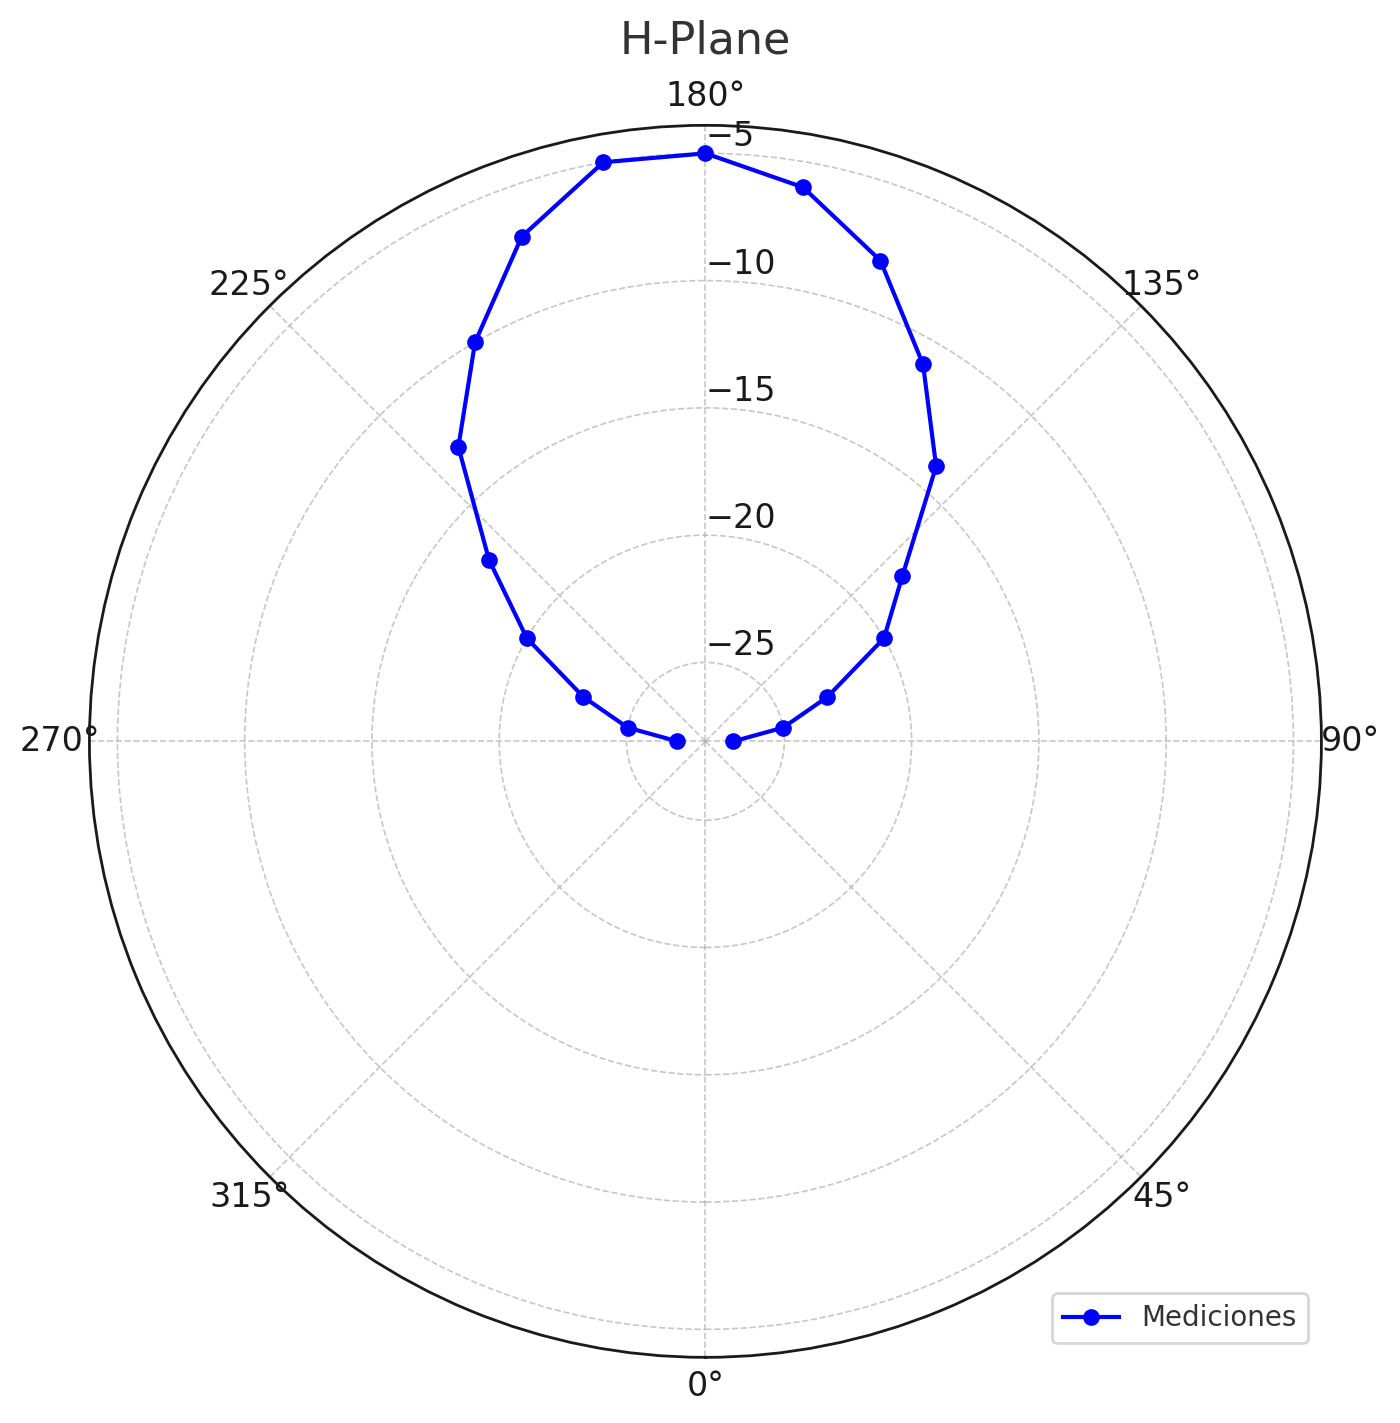
\includegraphics[width=0.4\textwidth]{img/ejemplos/Figure_10}
			\caption{Patron de radiacion en el plano H de la antena}
		\end{figure}
		\begin{figure}
			\centering
			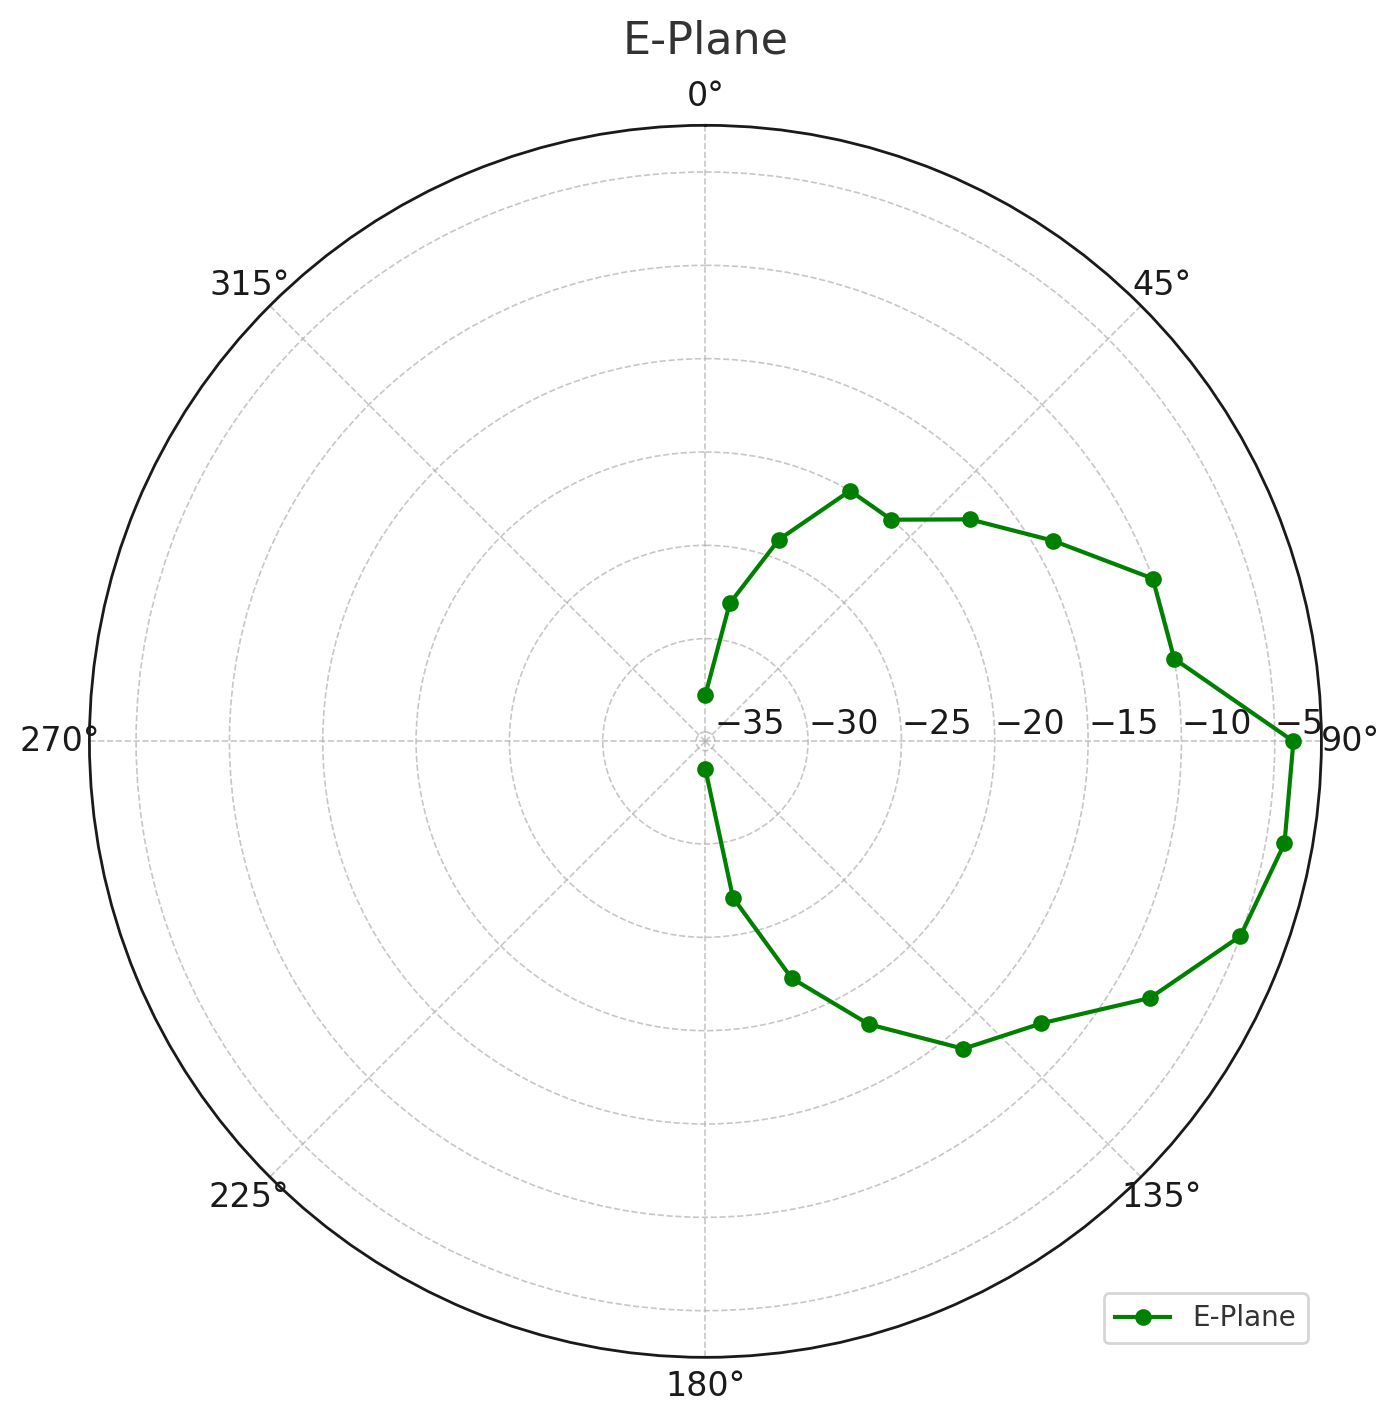
\includegraphics[width=0.4\textwidth]{img/ejemplos/Figure_11}
			\caption{Patron de radiacion en el plano E de la antena}
		\end{figure}
		Se observa un buen comportamiento en los patrones, con buena directividad, por lo que cumple con los requerimientos del proyecto.
		\newpage
		\item \textbf{Calcule la distancia mínima para encontrarse en el campo lejano de la antena parabólica. Ademas calcule la distancia necesaria para mantener libre la primera zona de Fresnell.}\\\\
		Para obtener la distancia minima para encontrarse en el campo lejano de la antena parabolica se utiliza la siguiente formula:
		\begin{align}
			R = \frac{2D^2}{\lambda}
		\end{align}
		Dado que se tiene que el diametro D de la antena parabolica corresponde a 59[cm] aproximadamente y que la frecuencia central es de 3.4[Ghz], reemplazando se obtiene que:
		\begin{align}
			\lambda = \frac{c}{f} = \frac{3*10^8}{3.4*10^9} = 0.088[m]
		\end{align}
		Reemplazando en la formula se obtiene que:
		\begin{align}
			R = \frac{2*(0.59)^2}{0.088} = 7.9[m]
		\end{align}
		Con lo que se obtiene que la distancia minima para encontrarse en el campo lejano de la antena parabolica es de 7.9[m]. Considerando lo anterior, se utilizo una distancia de aproximadamente 10[m] para las proximas mediciones.\\\\
		Luego para el valor de la primera zona de Fresnel tenemos que considerar la formula:
		\begin{align}
			F_{1} = \sqrt{\frac{\lambda \cdot d_{1} \cdot d_{2}}{d_{1} + d_{2}}}
		\end{align}
		Con lo que considerando que $d_{1} = d_{2}$ , se obtiene que :
		\begin{align}
			F_{1} = \sqrt{\frac{0.088 \cdot 5 \cdot 5}{10}} = 0.33[m]
		\end{align} 
		Con lo que se obtiene que la distancia necesaria para mantener libre la primera zona de Fresnell es de 0.33[m].
		\newpage
		\item{ \textbf{Mida el patrón de radiación (sistema completo) en ambos planos considerando un radioenlace copolarizado. Para conseguir el objetivo rote la antena en ambos ejes (Azimutal y Elevación)}}\\\\
		Se busca medir el patron de radiacion del sistema completo, para ello se procede a rotar la antena en ambos ejes, se obtiene los siguientes resultados en el eje Azimutal y un angulo de elevacion donde se tiene la maxima ganancia.
		\begin{figure}
			\centering
			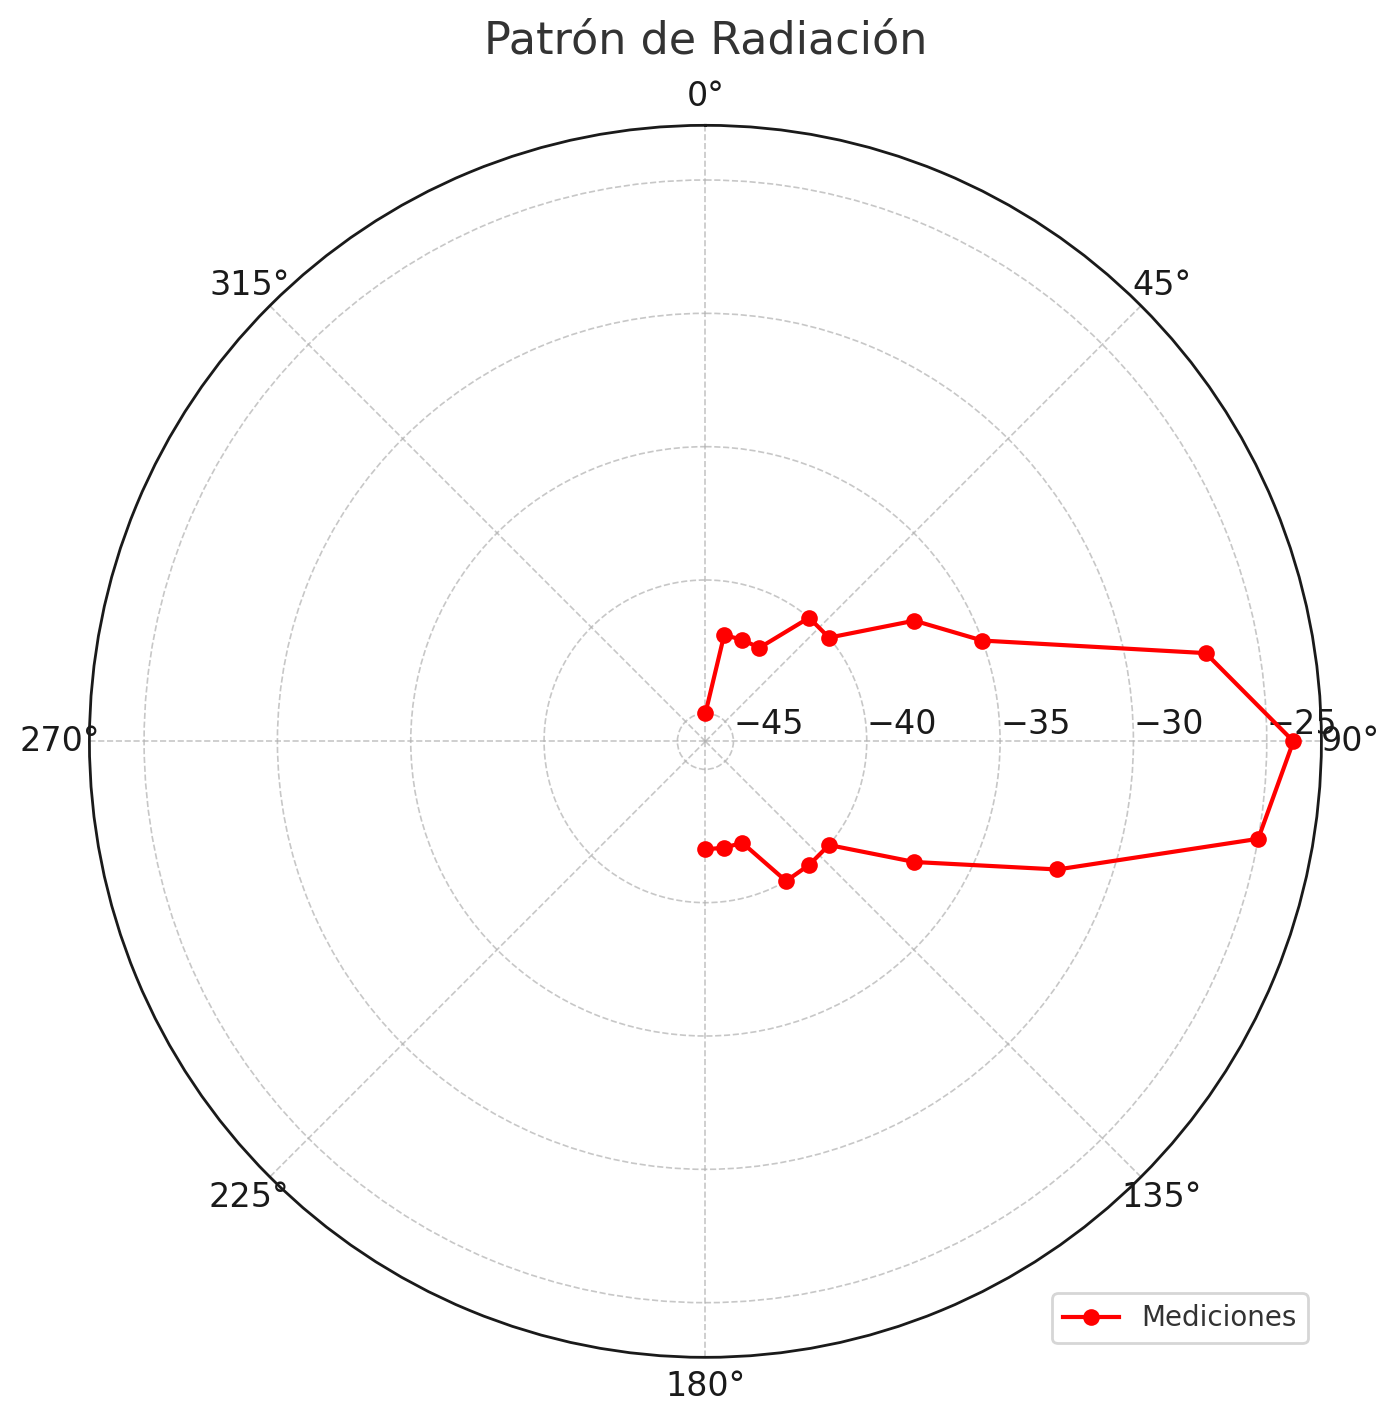
\includegraphics[width=0.5\textwidth]{img/ejemplos/Figure_12}
			\caption{Patron de radiacion en el eje Azimutal}
		\end{figure}
		Se observan buenos resultados en el patron de radiacion, similares a los obtenidos de manera teorica.
		\item{\textbf{Estime la Directividad y Ganancia del conjunto completo a partir de las mediciones.}}\\\\
		
		Se busca obtener la directividad y ganancia del conjunto completo a partir de las mediciones, para ello se utiliza la formula de Friss dada por:
		\begin{itemize}
			\item \(P_r (\text{dBm})\): Es la potencia recibida en la antena receptora. Su valor es \(-24 \, \text{dBm}\), obtenido anteriormente
			\item \(P_t (\text{dBm})\): Es la potencia transmitida desde la antena transmisora. Su valor es \(0.23 \, \text{dBm}\).
			\item \(G_t (\text{dB})\): Es la ganancia de la antena transmisora de la LPDA, que se asumira con un valor corresponde a \(7 \, \text{dB}\).
			\item \(G_r (\text{dB})\): Es la ganancia de la antena receptora que debemos calcular.
			\item \(R (\text{km})\): Es la distancia entre las antenas.Se asume de  \(10 \, \text{m}\), lo que equivale a \(0.01 \, \text{km}\).
			\item \(f (\text{MHz})\): Es la frecuencia de operación, que corresponde a \(3.4 \, \text{GHz}\), o \(3400 \, \text{MHz}\).
			\item \(P_{\text{cable}} (\text{dB})\): Representa la pérdida por el cable de transmisión. Sabemos que el cable tiene una pérdida aproximada de \(1 \, \text{dB/km}\) y que su longitud es de \(10 \, \text{m}\), resultando en \(0.01 \, \text{dB}\).
			\item \(P_{\text{amp}} (\text{dB})\): Es la amplificación adicional por los amplificadores. Nos indican que hay dos amplificadores con ganancias de \(16 \, \text{dB}\) y \(33 \, \text{dB}\), resultando en un total de \(49 \, \text{dB}\).
		\end{itemize}
		Luego utilizando la formula de Friss se tiene que:
		\begin{align*}
			P_r (\text{dBm}) &= P_t (\text{dBm}) + G_t (\text{dB}) + G_r (\text{dB}) \\
			&\quad - 20 \log R (\text{km}) - 20 \log f (\text{MHz}) \\
			&\quad - 32.44 - P_{\text{cable}} + P_{\text{amp}}.
		\end{align*}
			Sustituimos los valores conocidos:
			\begin{align}
			-24 &= 0.23 + 7 + G_r - 20 \log(0.01) - 20 \log(3400) - 32.44 - 0.01 + (16 + 33)
			\end{align}
			Tendremos por separado que los terminos vienen dados por:
			\begin{align}
			20 \log(0.01) &= 20 \cdot (-2) = -40 \, \text{dB}, \\
			20 \log(3400) &= 20 \cdot \log(3400) = 20 \cdot 3.5315 \approx 70.63 \, \text{dB}, \\
			P_{\text{cable}} &= -0.01 \, \text{dB}, \\
			P_{\text{amp}} &= 16 + 33 = 49 \, \text{dB}.
			\end{align}
			
			Sustituyendo nuevamente:
			\begin{align}
			-24 &= 0.23 + 7 + G_r - (-40) - 70.63 - 32.44 - 0.01 + 49.
			\end{align}
			
			Simplificamos los términos dentro del paréntesis:
			\begin{align}
			-24 &= G_r + (0.23 + 7 + 40 - 70.63 - 32.44 - 0.01 + 49).
			\end{align}
			
			Sumamos los valores numéricos:
			\begin{align}
			-24 &= G_r + (-6.85).
			\end{align}
			
			Despejamos \(G_r\):
			\begin{align}
			G_r &= -24 + 6.85, \\
			G_r &= -17.15 \, \text{dB}.
			\end{align}
			Se obtiene que la ganancia de la antena receptora es de \(-17.15 \, \text{dB}\). Por otro lado la directividad de manera directa se tiene que:
			\begin{align}
				D = \frac{4\pi A}{\lambda^{2}} \epsilon
			\end{align}
			Considerando que el plato de la antena parabolica tiene un diametro de 59[cm] y que la frecuencia de operacion es de 3.4[Ghz] y con un $\epsilon =0.65$ se logra obtener que:
			\begin{align}
				D = \frac{4\pi (1.2)}{(0.088)^{2}} 
			\end{align}
			En decibeles dando un valor aproximado de 31dB

\end{itemize}


